\subsection{Overview}
We need to design a system in which the user asks to the system to store an appointment and calculate the best path from a starting location to the appointment location. \\
Since this interaction between user and system can be summarize as:
\begin{enumerate}
	\item User request a service to the system.
	\item System responds to the user with the requested service.
\end{enumerate}
Based on this, we decide to use a client-server architectural approach.
\begin{figure}[H]
	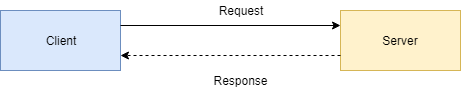
\includegraphics{Img/ClientServerArchitecture}
	\caption{Client Server architecture}
	\label{fig:clientserver}
\end{figure}
Furthermore, the system can be divided into three different subsystems: the presentation layer, the application layer and the data layer as we can see in \autoref{fig:overview}. 
\begin{itemize}
	\item The \emph{Presentation Layer} provides the GUI of the system. This layer contains
	the mobile application and the web pages.
	\item The \emph{Logic Layer} contains the logic of the application,that receives the requests from the user, computes the best path to reach the appointment, checks the weather and the road conditions and executes the dynamic web pages of the web site.
	\item The \emph{Data Layer} stores and maintains the data needed from the system to works properly, i.e. user’s information and user’s appointment information.
\end{itemize}
\begin{figure}
	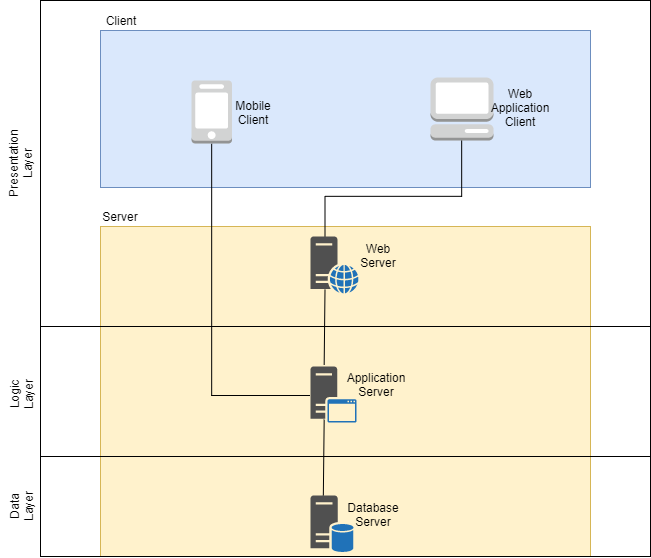
\includegraphics[width=\textwidth, height=\textheight, keepaspectratio=true]{Img/Overview}
	\caption{Overview of the system architecture}
	\label{fig:overview}
\end{figure}

\clearpage


\subsection{Component View}

\subsubsection{Overview}

In \autoref{fig:hlCD} is possible to see the high level components of the system and the interfaces used to connect one to another, where
\begin{itemize}
	\item the \emph{DBMS} provides the database and a way to retrieve data from it;
	\item the \emph{Application Server} provides the main logic of the application;
	\item the \emph{Web Server} provides the static pages and executes the dynamic pages of the web site.
	\item the \emph{Mobile Application} is the mobile application used by a user with his/her smartphone.
	\item the \emph{Web Application} is the application that runs on the user's browser.
\end{itemize}

\begin{figure}
	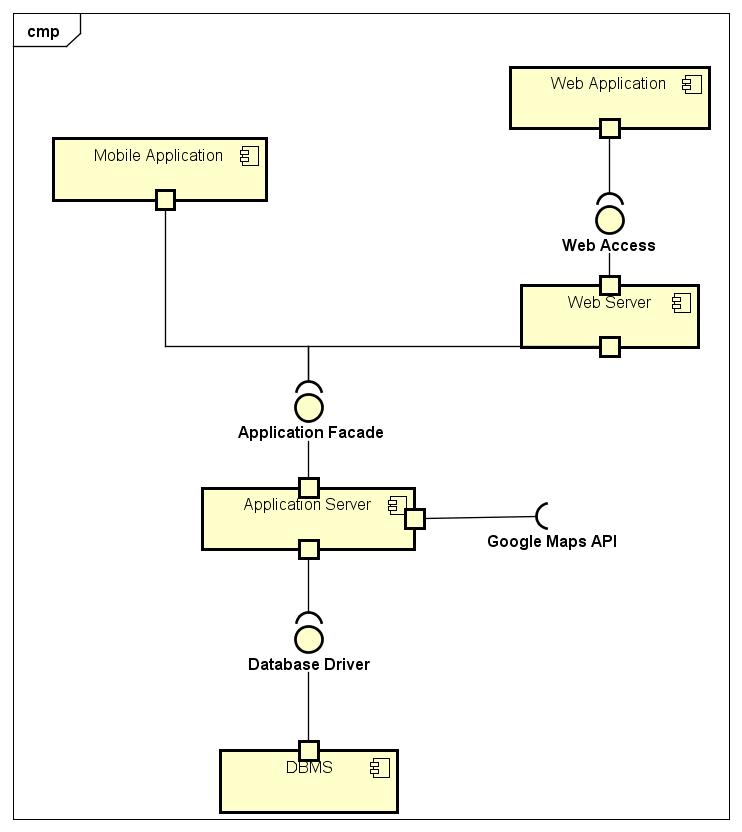
\includegraphics[width = \textwidth, keepaspectratio = true]{Img/HighLevelComponent}
	\caption{High level Component Diagram}
	\label{fig:hlCD}
\end{figure}

\subsubsection{Database View}
The DBMS component provides a database and is DBMS for data storage and their management.
It is possible to access the database only through the Application Server and an appropriate secure interface.
For security and privacy reasons, data are encrypted inside the database.
The Entity-Relationship diagram of the database is showed in \autoref{fig:ERDiagram}.

\begin{figure}
	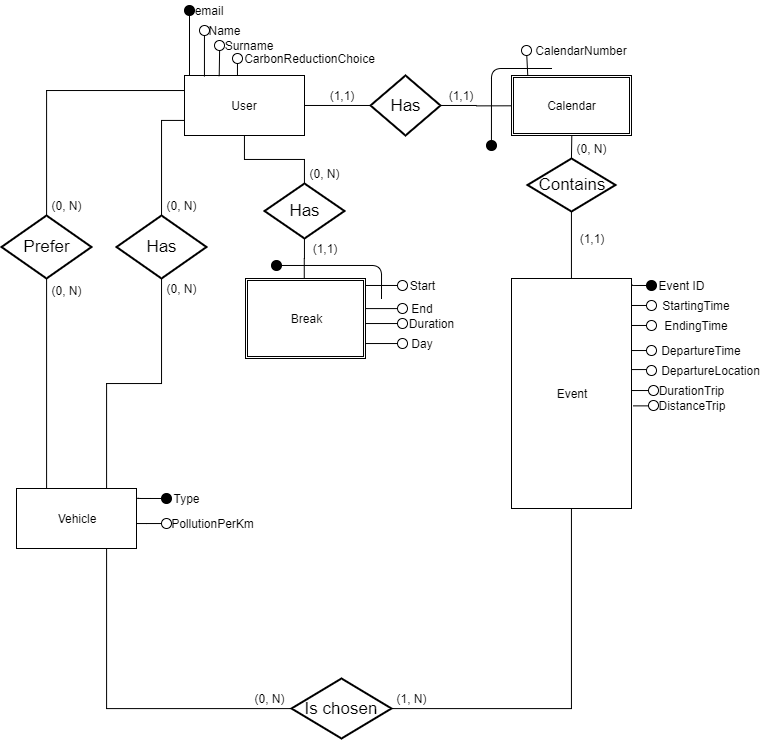
\includegraphics[width = \textwidth, keepaspectratio = true]{Img/ERDiagram}
	\caption{\emph{Entity-Relationship Diagram} of the database}
	\label{fig:ERDiagram}
\end{figure}

\subsubsection{Application Server View}
The \emph{Application Server} contains the main logic of the application. It receives the user's request and interacts with the database to store and retrieves data. 
The \emph{Application Server} as we can see in \autoref{fig:applicationservercomponentCD} is composed of:

\begin{itemize}
	\item \textbf{Authentication Manager}, it manages the request of a user to register or to login into the service. It can access to \emph{Account Data Manager} to retrieves user's information from the database.
	\item \textbf{Profile Manager}, it manages the request of a user to update his/her profile. It can access the \emph{Account Data Manager} in order to retrieves information in the database.
	\item \textbf{Account Data Manager}, it can access all the information about the user's account in the database. 
	\item \textbf{Appointment Manager}, provides to the user the functionalities of creation / modification of appointments. It uses the \emph{Path Calculator} to obtain the best path for the appointment and the \emph{Appointment Data Manager} to stores and retrieves information.
	\item \textbf{Path Calculator}, it is responsible to compute the best path from the starting location defined by the user and the appointment location. To do so, it can access the \emph{Additional Info Facade} to retrieves the user preferences, the weather and road informations. It needs also the \emph{Google Maps API} to retrieves distance and time informations.
	\item \textbf{Weather Information Manager}, it manages weather information retrieving it from an external system via its API, showed in the diagram as \emph{Weather API}.
		\item \textbf{Road Information Manager}, it manages road information retrieving it from an external system via its API, showed in the diagram as \emph{Road API}.
	\item \textbf{Additional Info Facade}, it is a component that implements the \emph{Facade Pattern}, in this way it is possible to reduce the coupling between the \emph{Path Calculator} and the other interfaces from that needs to get information required.
	\item \textbf{Travlendar+ Facade}, it is a component that implements the \emph{Facade Pattern} and provides a common interface for both the \emph{Mobile Application} and the \emph{Web Server}.	
\end{itemize}

\begin{figure}
	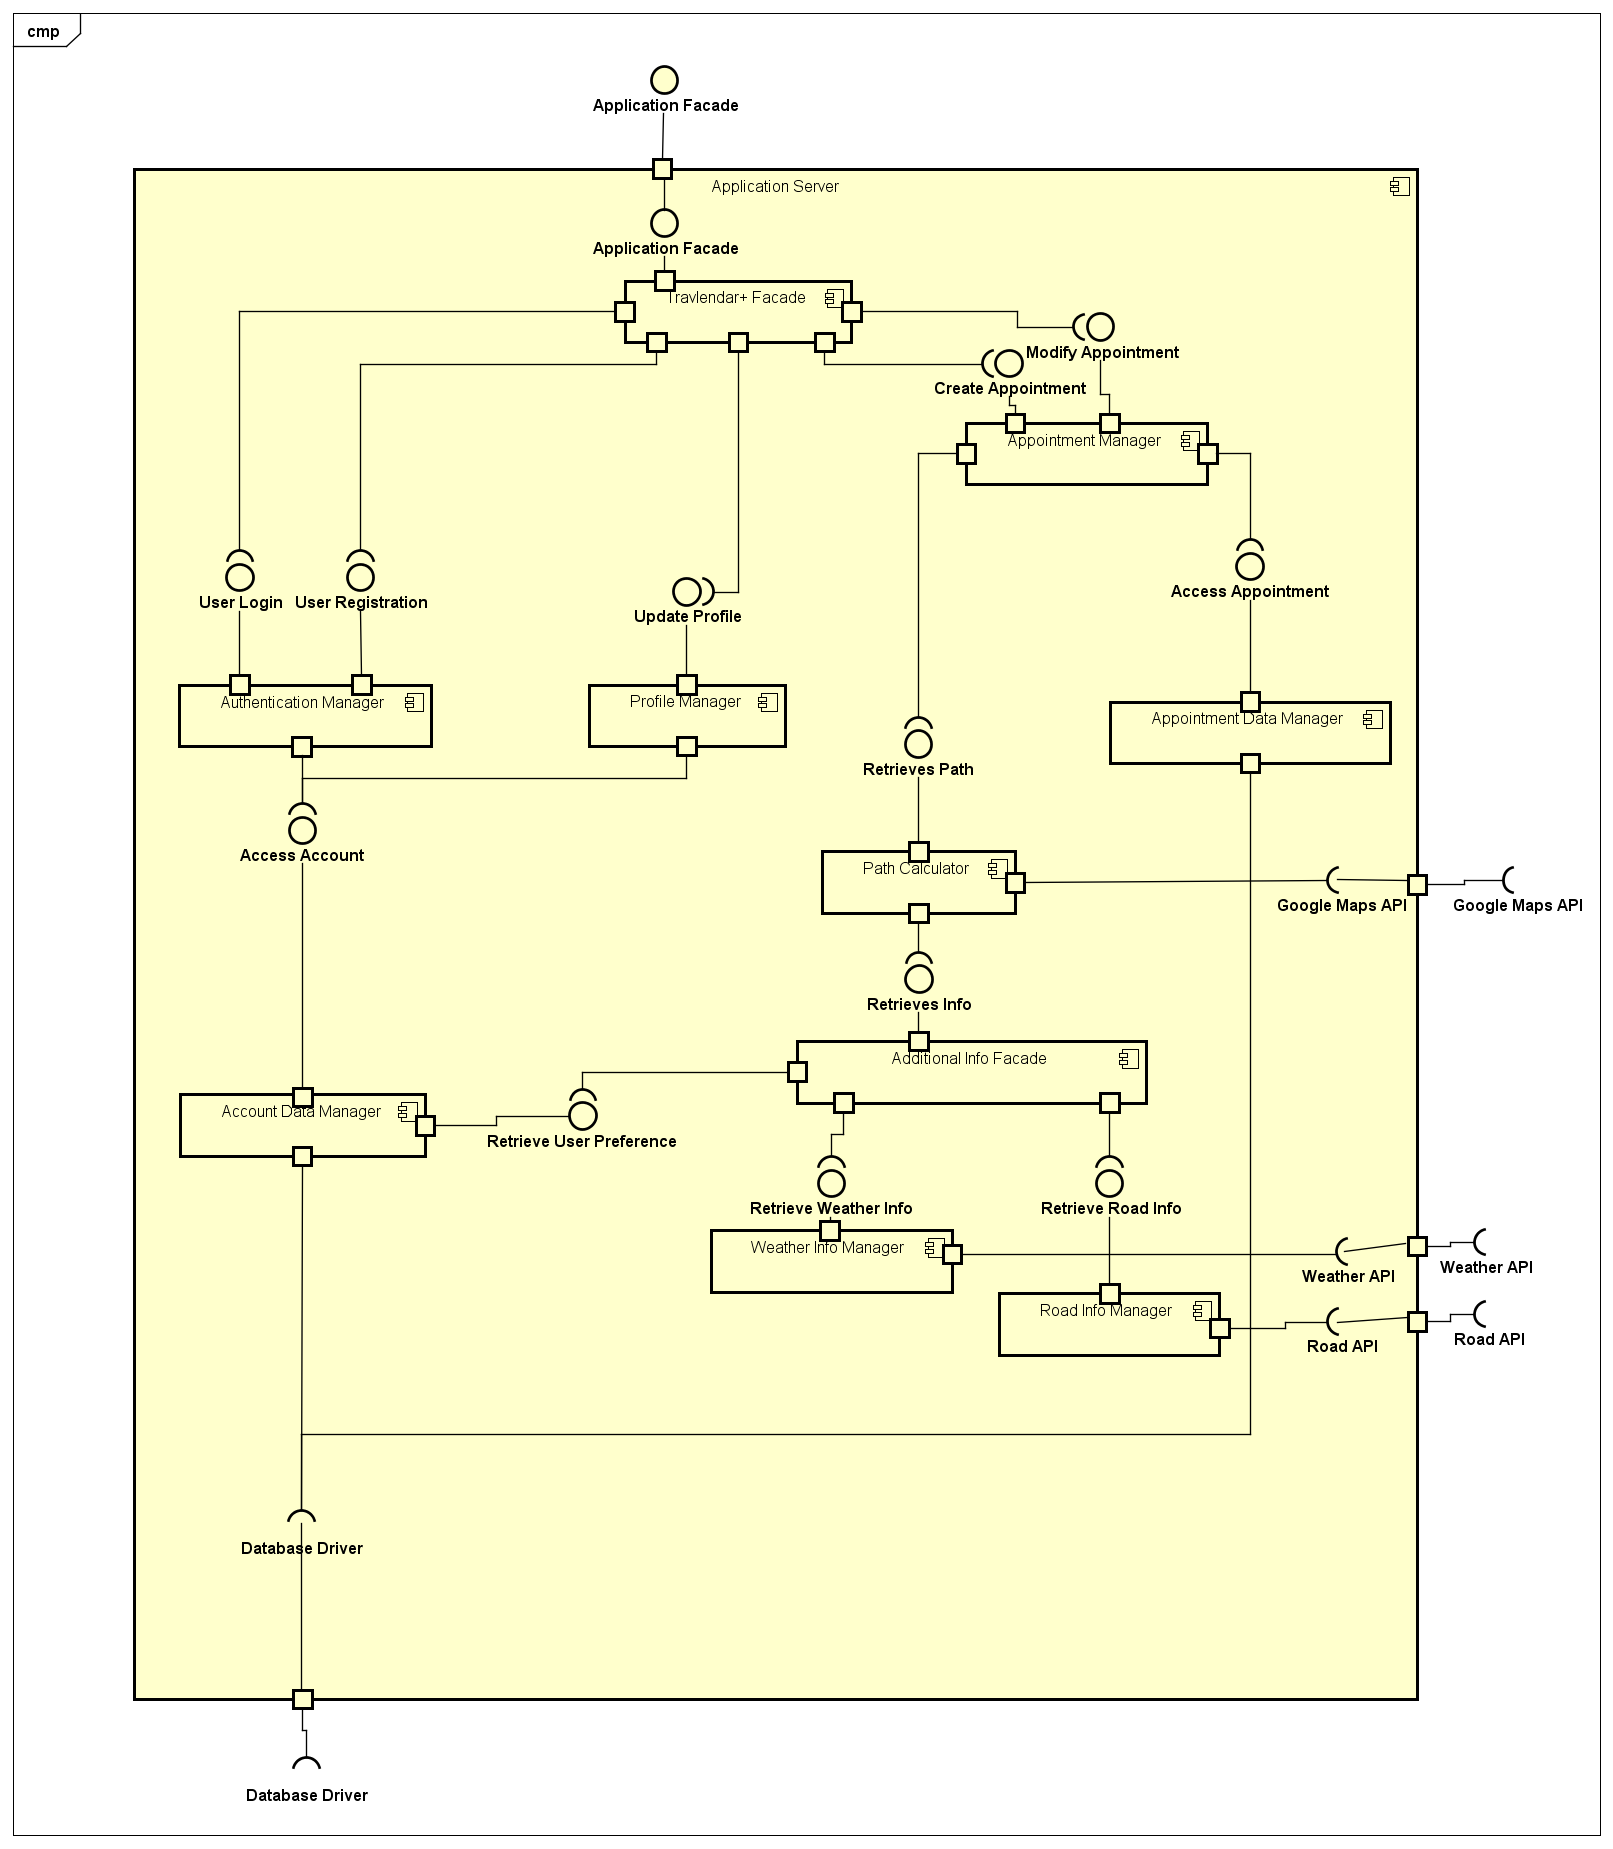
\includegraphics[width = \textwidth, height = \textheight, keepaspectratio = true]{Img/ApplicationServerCD}
	\caption{\emph{Application Server} component diagram}
	\label{fig:applicationservercomponentCD}
\end{figure}

\subsubsection{Web Server}
Since the presence of a \emph{Web Application}, it is necessary a dedicated \emph{Web Server} responsible to executes the web site’s dynamic pages and provides the static pages to the user’s browser.
The \emph{Web Server} interacts with the \emph{Application Server} to get the proper information to fill up the pages.
The \emph{Web Server} also sends data from the user’s browser to the \emph{Application Server} to store inside the database.

\subsubsection{Mobile Application}
The \emph{Mobile Application} is used by the user via its own smart device. The \emph{Mobile Application} communicates directly the \emph{application server} with a dedicated communication protocol.
The component diagram of the \emph{Mobile Application} is showed in \autoref{fig:mobileapplicationCD}.
The description of the components is the follow:
\begin{itemize}
	\item \textbf{User View} is responsible of the graphical representation of the app and the interactions with the user.
	\item \textbf{GPS Manager} is responsible to interact with the GPS Module of the smart device.
	\item \textbf{DBMS}, is a physical view of the main database while storing only the current user's data.  It is used by the \emph{Controller} to notify the user when an event is about to start.
	\item \textbf{Controller}, is responsible to interact with the \emph{Application Server} and link together the other components.
\end{itemize}

\begin{figure}
	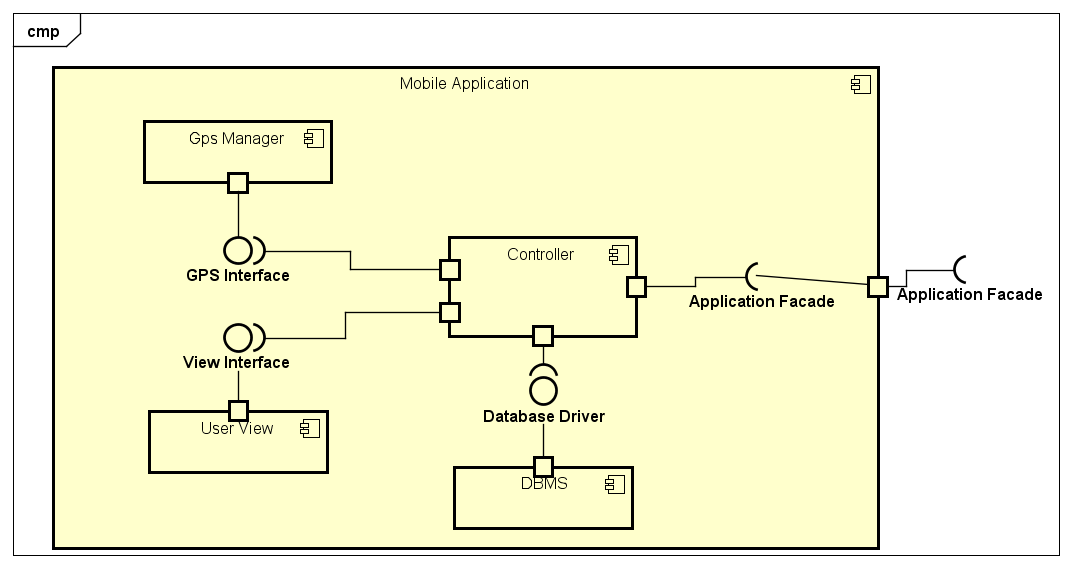
\includegraphics[width = \textwidth, keepaspectratio = true]{Img/MobileApplication}
	\caption{\emph{Mobile Application} component diagram}
	\label{fig:mobileapplicationCD}
\end{figure}

\clearpage
\subsection{Deployment View}
\label{DeploymentView}
The architecture chosen for Travlendar+ is a Four-Tier in Three-Layer one, where a high-level mapping layer to component is as follows:
\begin{itemize}
\item Presentation Layer: Mobile application/Web application and Web Server
\item Logic Layer: Application server
\item Data Layer: DBMS and Database
\end{itemize}
Note that the definition of layer is just a logic separation of the components that compose the system with the intent to better organise the code that needs to be developed, while a tier is a physical machine onto where the code is running.
\\To better understand the choice made a scheme is provided in \autoref{fig:TierLayerDiagram}, where it's clear that there are three layers (the different coloured boxes) and four physical tiers (We consider the mobile and web application as a single tier, while obviously the code is written in the DBMS and not in the DB).
\begin{figure}[h]
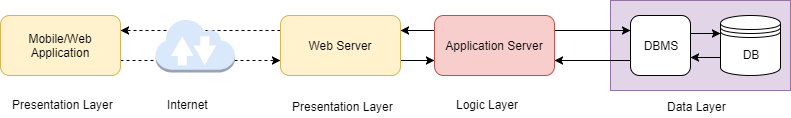
\includegraphics[width = \textwidth, keepaspectratio = true]{Img/TierLayerDiagram}
	\caption{System's Tiers and Layers}
	\label{fig:TierLayerDiagram}
\end{figure}
\paragraph*{Implementation choices\\}
The technology chosen for the implementation on the system are mainly based on Java Enterprise Edition (JEE) since it offers a large number of tools and alternatives to develop multi-tier systems that need web based logic and storage and having at the same time the possibility of adding new functionalities in future, making the system more scalable.\\
\textbf{Web Pages:} The choice fell on JSP given the flexibility that a few snippets of Java code in a dynamic web page can provide.\\
\textbf{Application Logic:} EJB was the selected technology given that the system is developed mainly using JEE.\\
\textbf{Application Server:} GlassFish 5.0 has been chosen over other alternatives since it's an open source application server fully supported by Oracle.
\textbf{Web Server:} GlassFish 5.0 was chosen again for coherence with the application server.\\
\textbf{DBMS}: MySQL was selected given that is supported by Oracle and is well known, making the amount of documentation available quite large. It was paired with InnoDB because it's the currently most used alternative and allows us to use foreign keys.\\

A complete overview of the technologies chosen can be seen in the decision flow diagram in \autoref{fig:DecisionFlow}
\begin{figure}
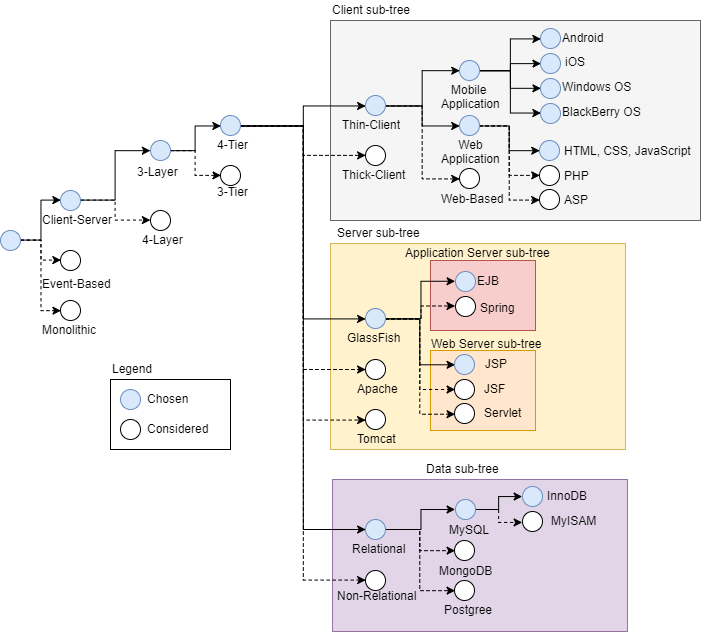
\includegraphics[width = \textwidth, keepaspectratio = true]{Img/DecisionFlow}
	\caption{Decision Flow Diagram}
	\label{fig:DecisionFlow}
\end{figure}
\newpage

\begin{samepage}
\subsubsection{Deployment Diagram}
The deployment diagram can be seen in \autoref{fig:DeploymentDiagram}, note that the components specified in \autoref{fig:mobileapplicationCD} and in \autoref{fig:applicationservercomponentCD} can be seen in this representation of the mapping on concrete devices.
\begin{figure}[h]
\centering
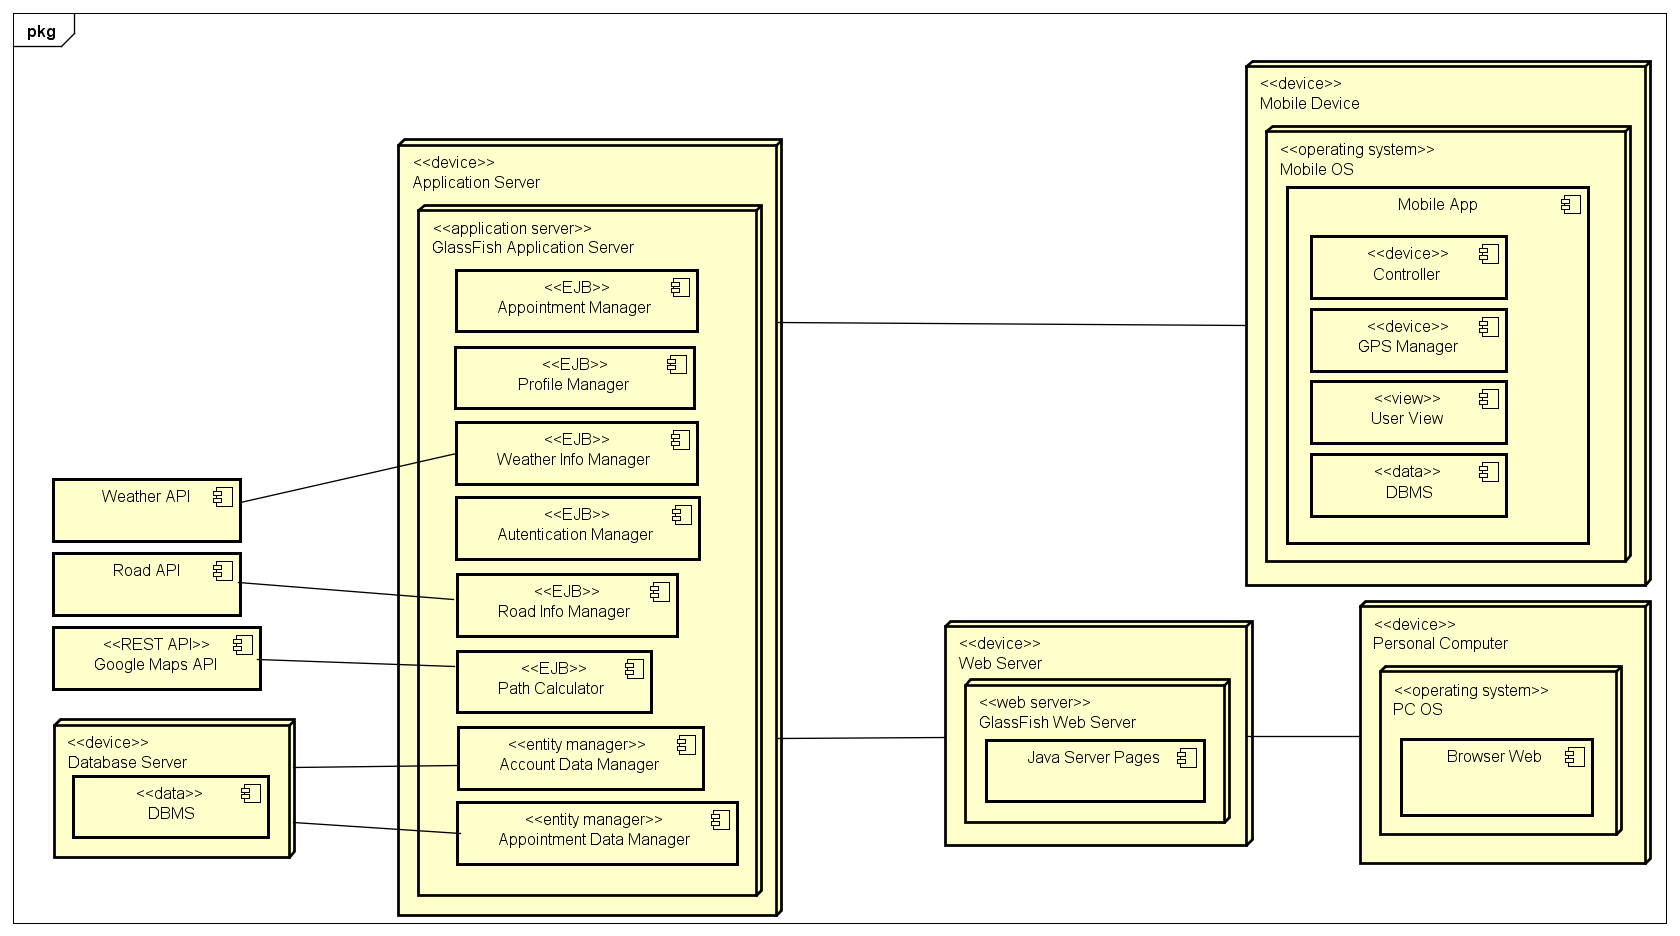
\includegraphics[scale=0.40, angle=90]{Img/DeploymentDiagram}
\caption{Deployment Diagram}
\label{fig:DeploymentDiagram}
\end{figure}
\end{samepage}

\clearpage
\subsection{Runtime View}
In this section are represented the most important runtime views by using sequence diagrams that highlight the main interactions between the user and the components of the system for each analysed use case.\\
Note that each \emph{Error Message} is just an abstraction of different errors with different codes for different situations, this was done in order to simplify the diagrams.

\begin{figure}
\centering
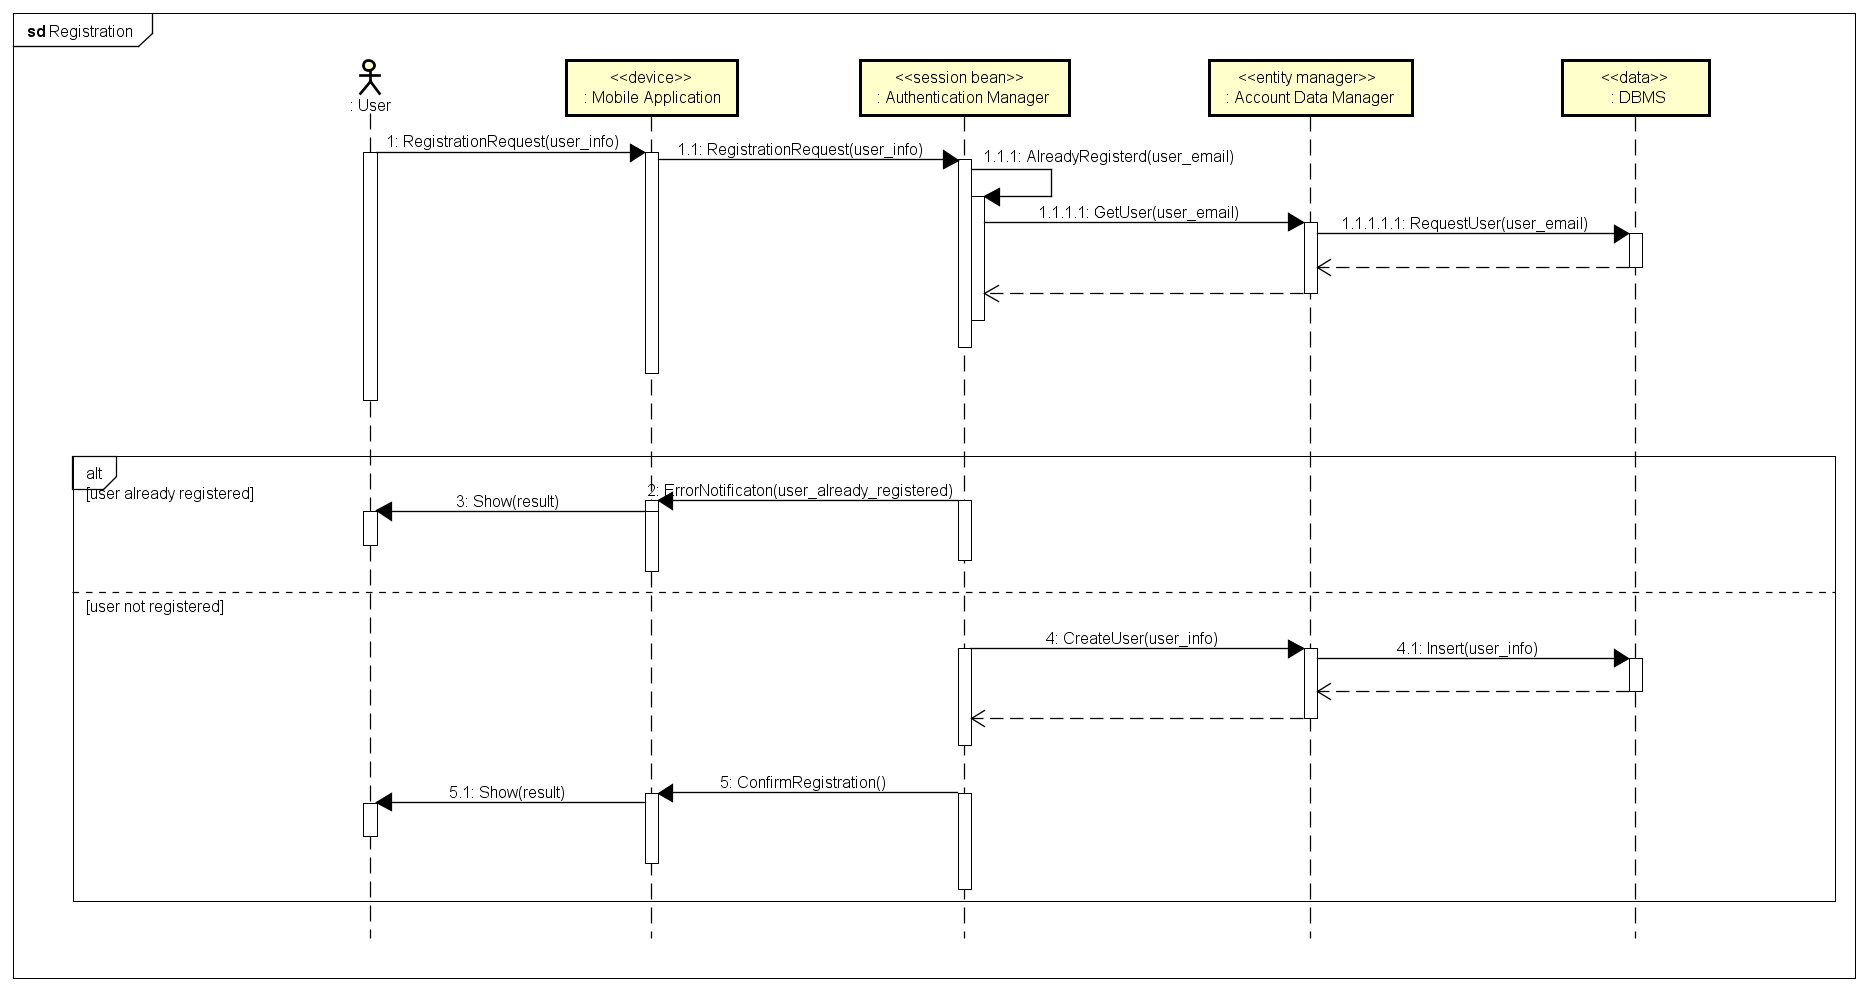
\includegraphics[width = \textwidth, keepaspectratio = true, angle=90]{Img/RegistrationSQ}
\caption{Diagram of interaction between components in the \emph{Registration} use case}
\label{fig:RegistrationSQ}
\end{figure}

\begin{figure}
\centering
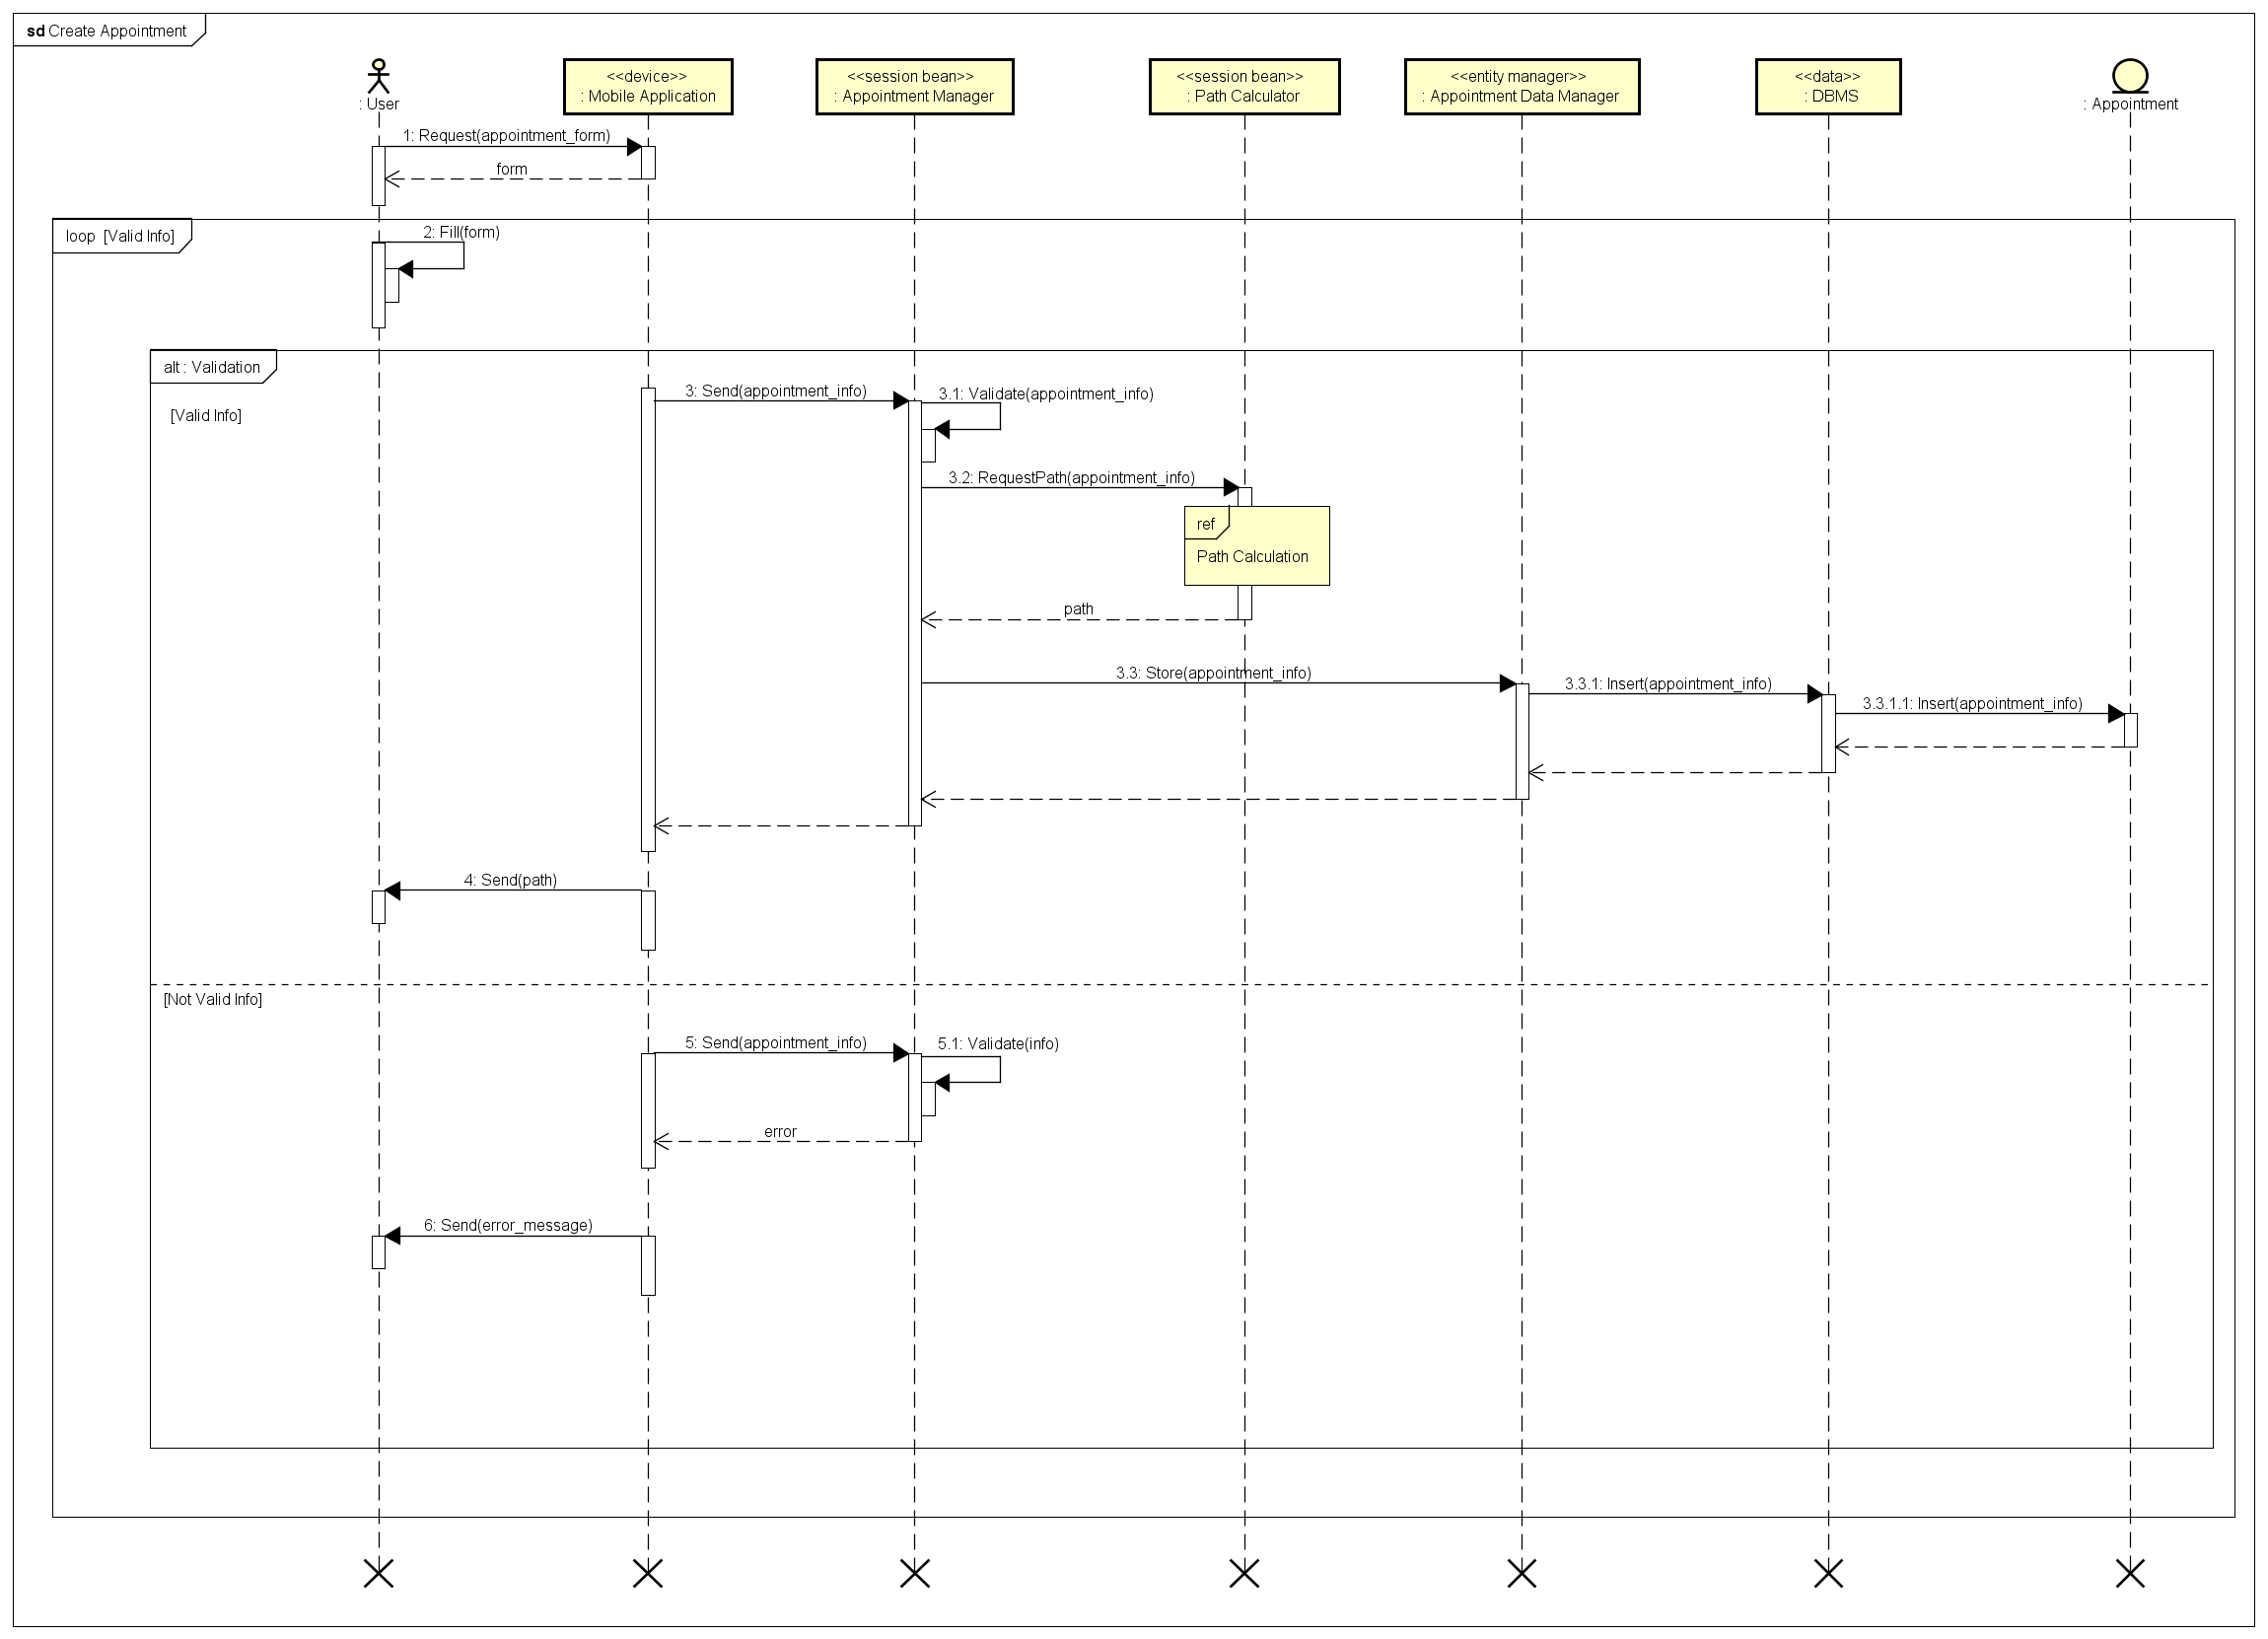
\includegraphics[width = \textwidth, keepaspectratio = true, angle=90]{Img/CreateAppointmentSQ}
\caption{Diagram of interaction between components in the \emph{Create Appointment} use case, the internal interaction of the path calculator is in \autoref{fig:PathCalculator}}
\label{fig:CreateAppointmentSQ}
\end{figure}

\begin{figure}[h]
\centering
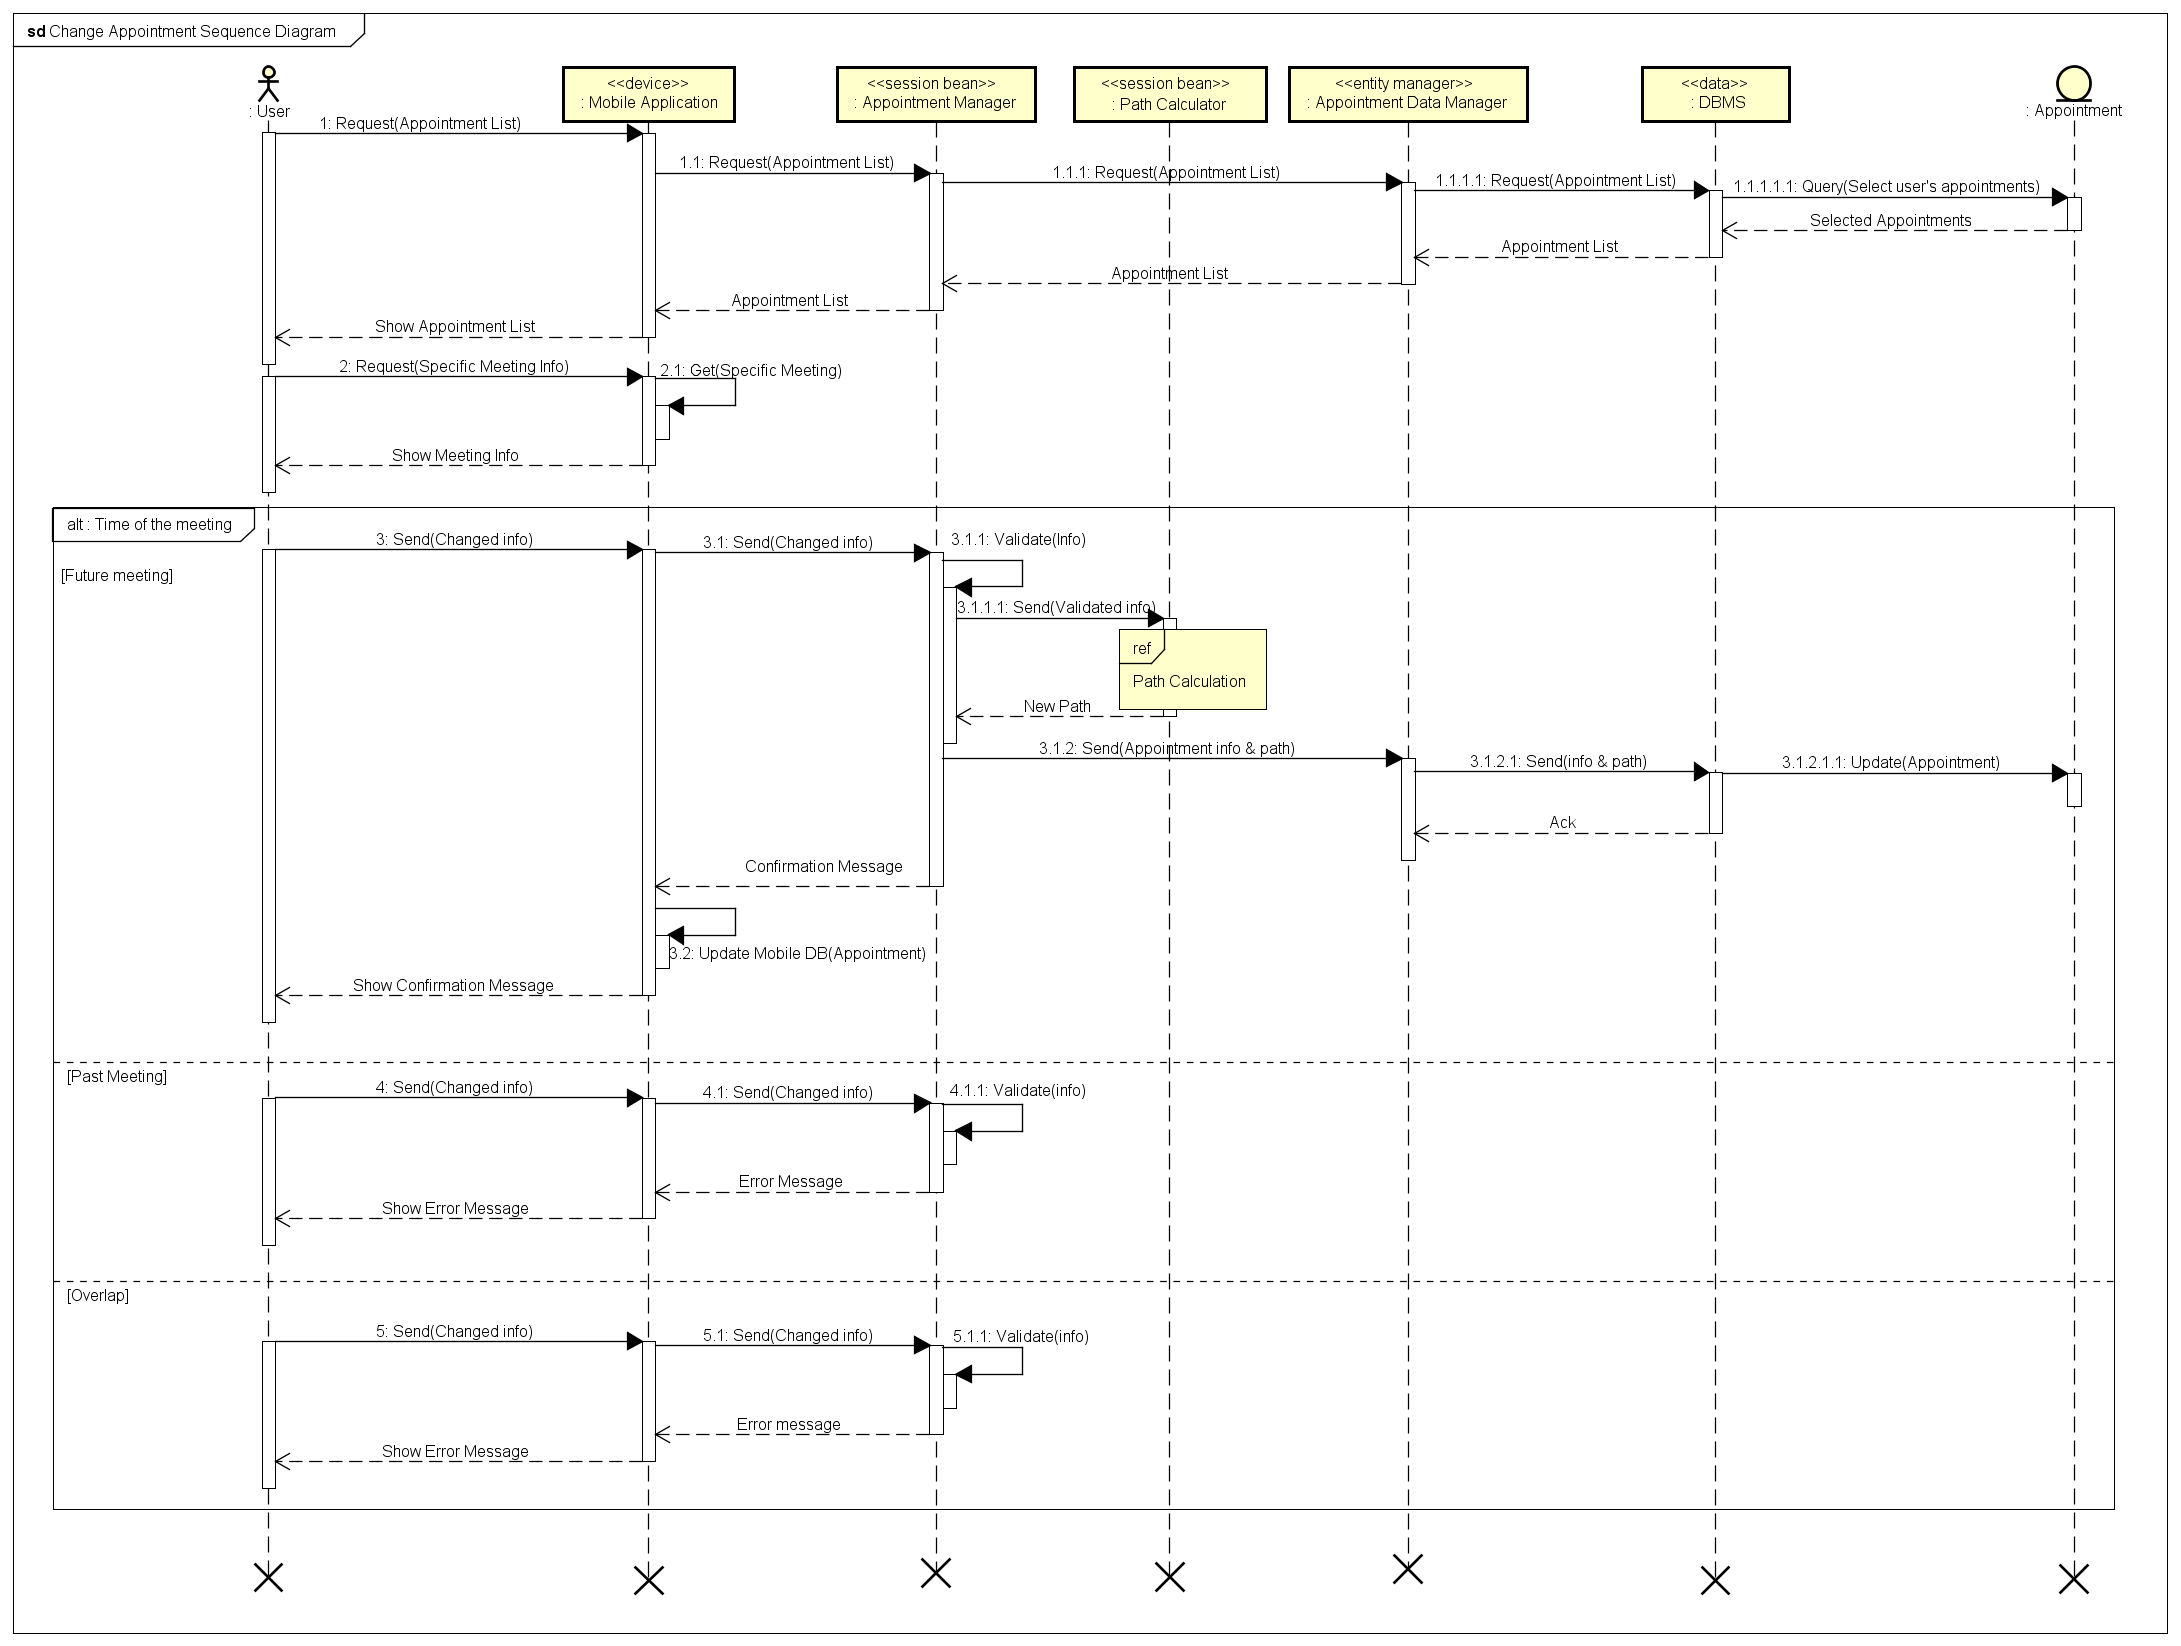
\includegraphics[width = \textwidth, keepaspectratio = true, angle=90]{Img/ChangeAppointmentSequence}
\caption{Diagram of the interaction between components in the \emph{Change Appointment} use case, it should be noted that the internal interaction of the path calculator is better specified in \autoref{fig:PathCalculator} in order to keep the diagram as clean as possible}
\label{fig:ChangeAppointmentSequence}
\end{figure}

\begin{figure}[h]
\centering
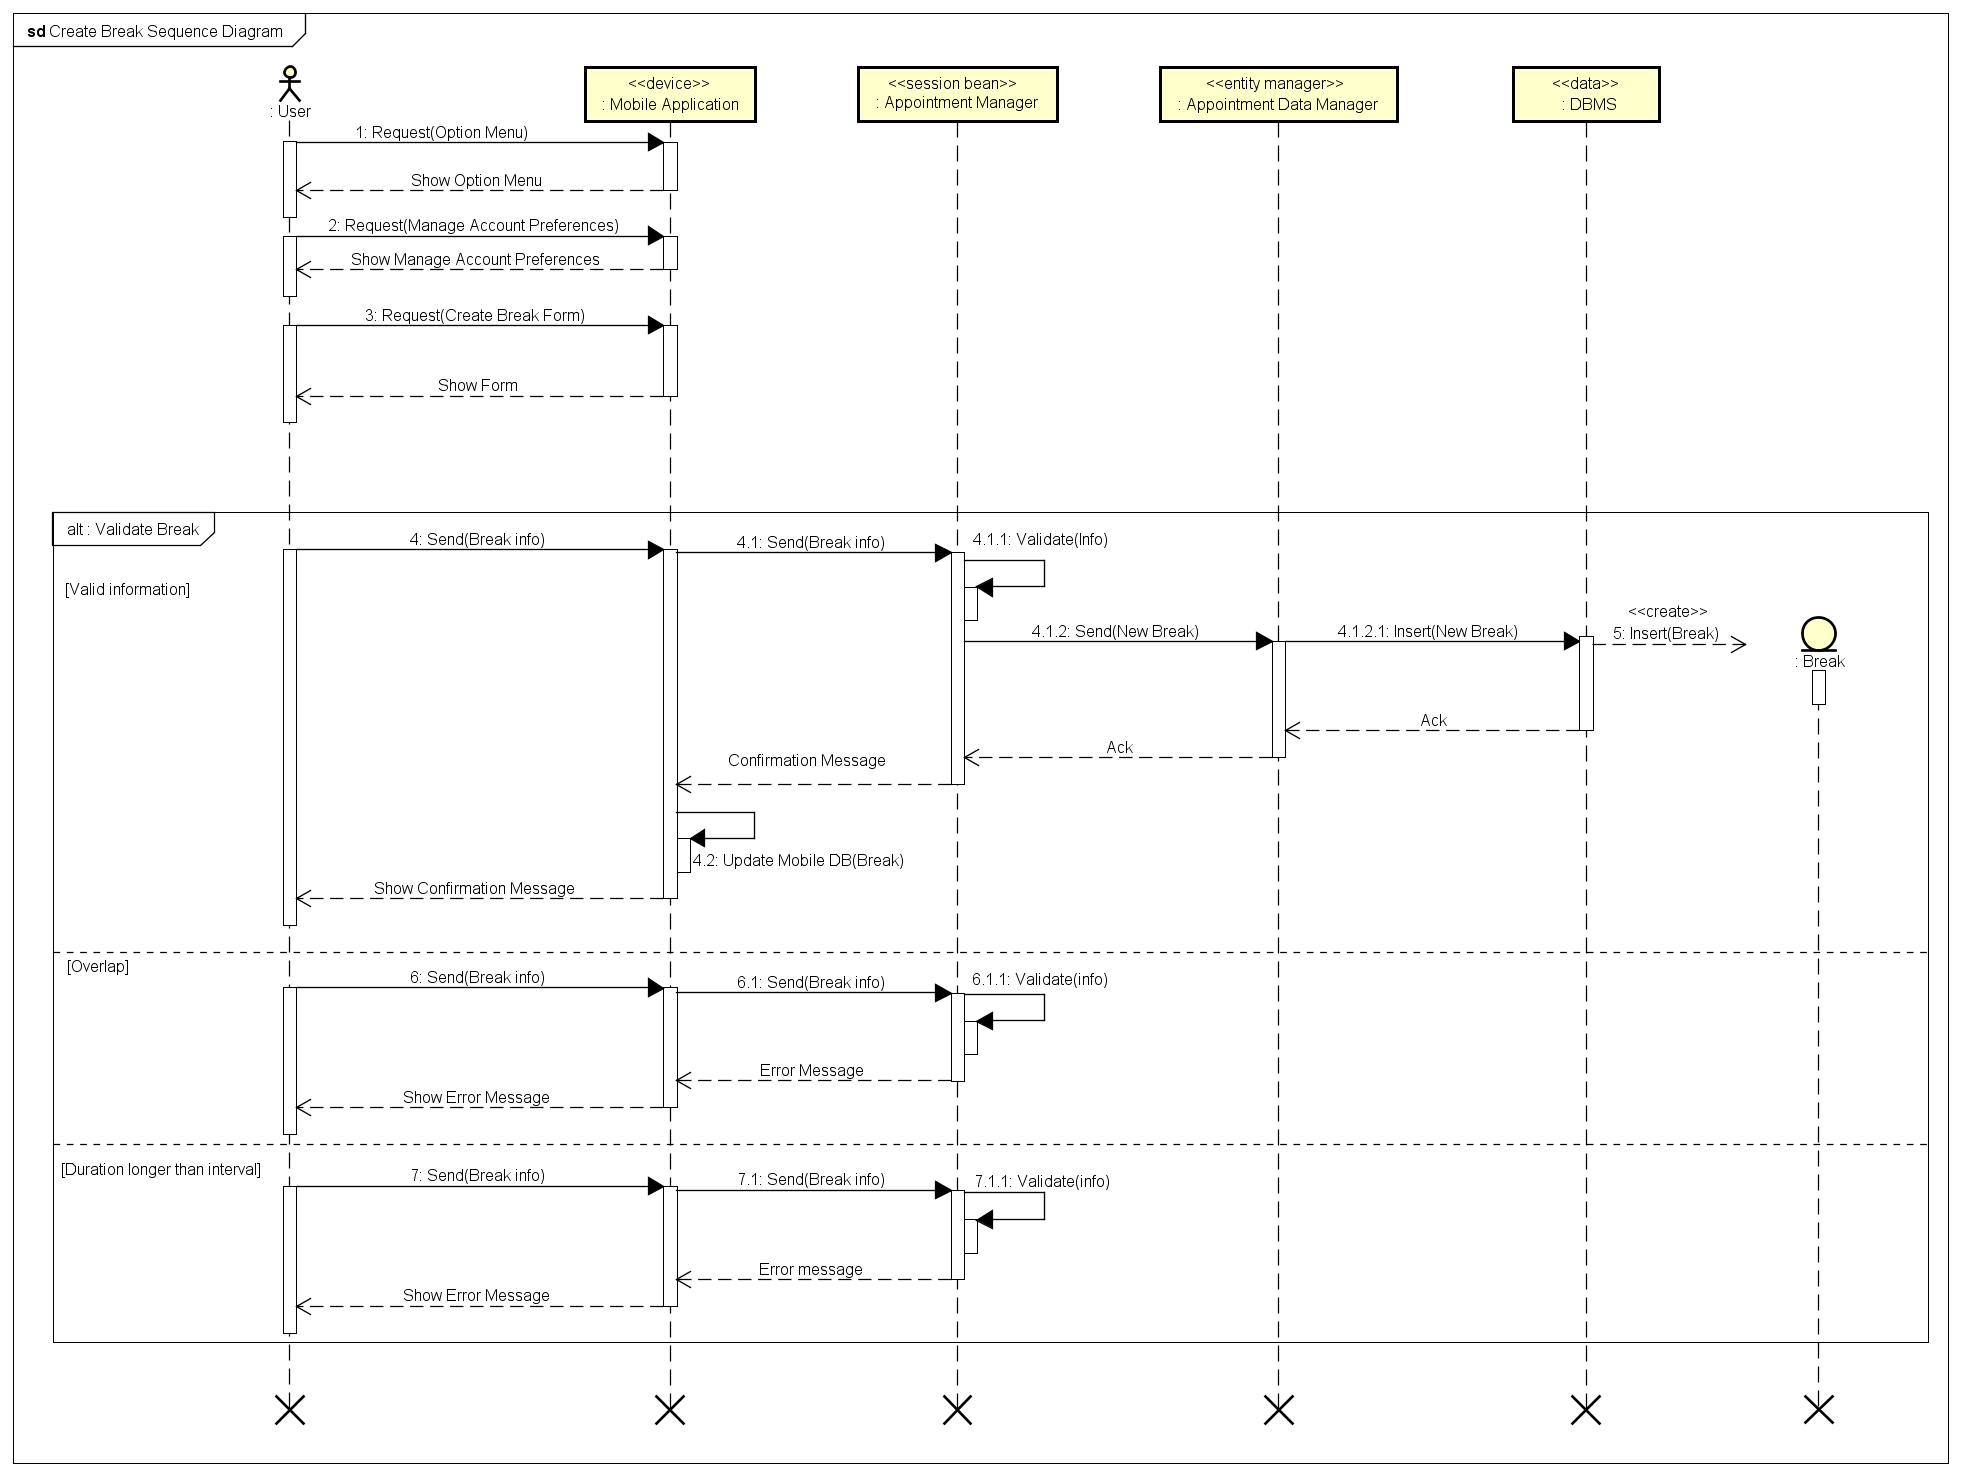
\includegraphics[width = \textwidth, keepaspectratio = true, angle=90]{Img/CreateBreakSequence}
\caption{Diagram of the interaction between components in the \emph{Create Break} use case, the \emph{AppointmentManager} manages also breaks}
\label{fig:CreateBreakSequence}
\end{figure}

\begin{figure}
\centering
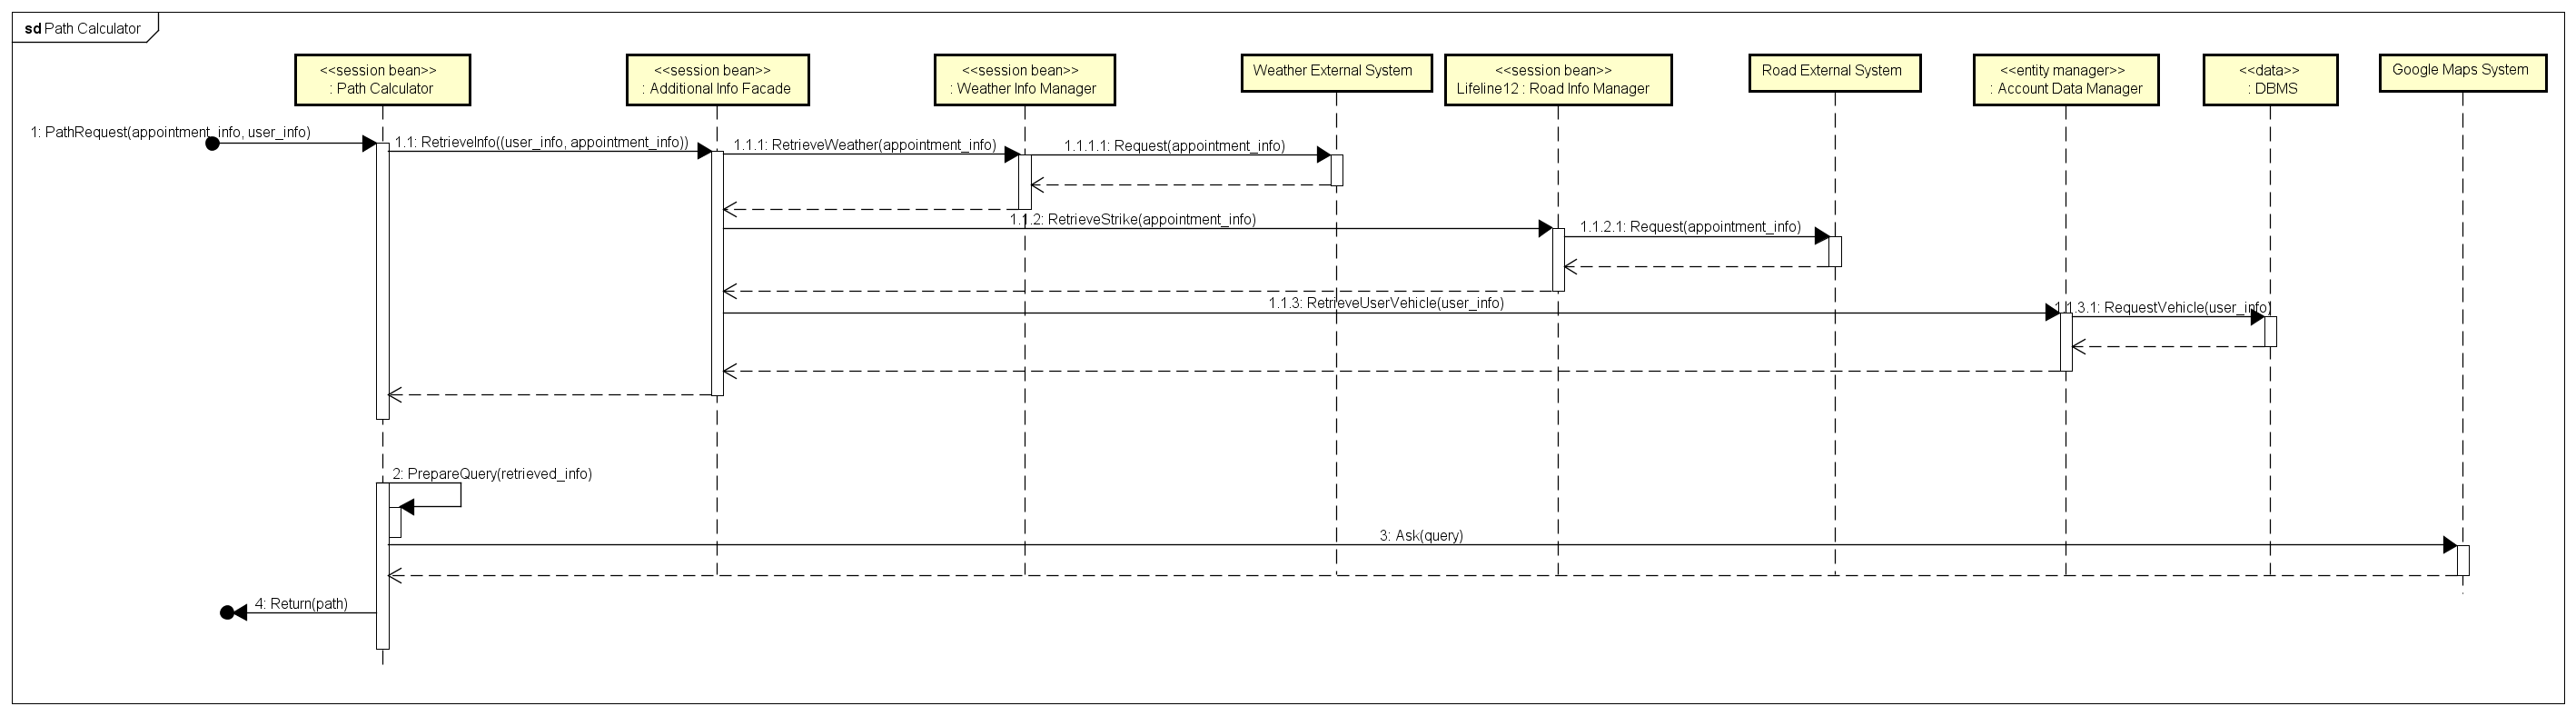
\includegraphics[width = \textwidth, keepaspectratio = true, angle=90]{Img/PathCalculator}
\caption{Diagram of the interaction between components during a calculation of a path.\\
The \emph{Path Calculator} asks for information to the \emph{Additional Info Facade}, and, based on this information, prepare the request to send to \emph{Google Maps}}
\label{fig:PathCalculator}
\end{figure}

\clearpage
\subsection{Communication Interfaces}
\subsubsection{Database Driver}
This interface is used to allows the interaction between the \emph{Application Server} and the \emph{DBMS}.\\
There are two different components that interacts with this interface:
\begin{itemize}
	\item Account Data Manager, for managing user's information.
	\item Appointment Data Manager, for managing appointments' information.
\end{itemize}

\subsubsection{Application Facade}
This interface provides a common point of access for both the \emph{Mobile Application} component and the \emph{Web Server} component.\\
It is provided form the \emph{Travlendar+ Facade}.

\subsubsection{Google Maps API}
This interface can provide:
\begin{itemize}
	\item a map of the path from the departure location to the appointment location.
	\item the ETA with a specific travel means
	\item the path directions for each travel means.
\end{itemize}
The \emph{Path Calculator} component builds the path from the information retrieved from this API.

\subsubsection{Weather API}
This interface provides a way to obtain the forecast of the appointment date.
The \emph{Path Calculator} component relies on this informations to take decision about the best path.

\subsubsection{Road API}
This interface provides a way to obtain information about possible strikes on the appointment date.
The \emph{Path Calculator} component relies on this informations to take decision about the best path.

\clearpage
\subsection{Selected architectural styles and patterns}
In this section we will discuss which architectural styles and were chosen and why.
\subsubsection{Client-Server}
The client-server architecture has been used multiple times, we note them all in the following list.
\begin{enumerate}
\item The \textbf{mobile application} is the client with regard to the \textbf{application server} (which is of course the server) that handles the requests, this ensures that the mobile application needs the least amount of logic programmed, we will elaborate more on this topic in \autoref{ThinClient}.
\item The \textbf{web browser} installed onto the user's personal computer acts as a client, while the server is the \textbf{web server} that receives its requests.
\item The \textbf{web server} is also a client when looking at its relationship with the application server, that has to handle the requests that are sent to the \textbf{web server} from the \textbf{web browser}.
\item The \textbf{application server} acts like a client too, this appends when it is performing query requests to the \textbf{DBMS} that is the server in the interaction.
\end{enumerate}

\subsubsection{Multi Tier}
Already discussed at the start of \autoref{DeploymentView}, a multi tier architecture allows the system to be much more \textbf{scalable} since each physical upgrade can be done without needing an intervention on the entire system.\\
It should be noted that it also benefits \textbf{fault tolerance} given that the mobile application can function without the need of the web server and it's \textbf{less expensive} to have redundant smaller section of the system rather than duplicating a mainframe.

\subsubsection{Thin Client}
\label{ThinClient}
A thin client architecture allows us to develop client side applications and interfaces that do not rely on the computational power of the user's hardware, this means that the system will be accessible even to users that do not own powerful last generation devices , this way the logic of the system is handled entirely by the application server, while the client side applications need only to display the information received from the server side, an abstract representation of the thin client concept can be seen in \autoref{ThinClient}.
\begin{figure}[h]
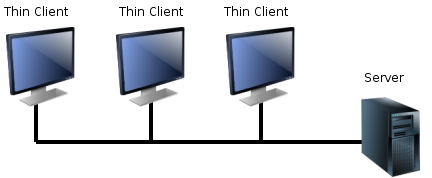
\includegraphics[]{Img/ThinClients}
\caption{A series of thin clients connected to a server that provides the computational power.}
\label{ThinClient}
\end{figure}

\clearpage
\subsection{Other design decision}
\subsubsection{Google Maps}
Given that for a project of this size is not feasible to develop and maintain an entire navigation system, we will rely on \emph{Google Maps} given the extreme flexibility that its APIs offer.\\
This choice translates in a path calculator that will act more like a \textit{builder for queries}, as it will be discussed more in detail when talking about the algorithms used.

\subsubsection{Cryptography}
Given that the system has to memorize date, place and travel of the user for each event, privacy concerns can arise.\\
The system uses the \textbf{Advanced Encryption Standard} (AES) used as a standard by the U.S.A. government in the stronger 256 bits cipher to protect the user's most sensible information (like email and password) and the quicker 128 bits one for the trips data.\\
Using the method just described the system can still process with relative ease the tasks it is asked to do and even if a brute-force attack could manage to extract information about a trip, the identity of the user would still be almost impossible to decipher before it's obsolete.\\
Periodic re-ciphering of information is also scheduled when the traffic flow in the system is low.














